The non-relativistic, Coulomb-interaction only Hamiltonian for \h\ is given by 
\begin{equation}
\label{eq:H}
H = \frac{p_1^2}{2m_e} + \frac{p_2^2}{2m_e} - \frac{1}{4\pi\epsilon_0}\frac{e^2}{r_1} -  \frac{1}{4\pi\epsilon_0}\frac{e^2}{r_2} +  \frac{1}{4\pi\epsilon_0}\frac{e^2}{r_{12}}
\eeq
where $m_e$ is the mass of the electron, $p$ is the classical kinetic energy of the electron specified by the subscript, $e$ is the charge of the electron, $\epsilon_0$ is the vacuum permittivity, $r_1$ is the distance from the first electron to the nucleus, $r_2$ is the corresponding value for the second electron, and $r_{12}$ is the distance between the two electrons.  In this Hamiltonian the nucleus is assumed to be fixed and thus does not possess its own kinetic energy.  This Hamiltonian possesses a term for each electron's kinetic energy, each electron's potential energy from its interaction with the nucleus (a single proton), and (specifically the last term in equation~\ref{eq:H}) a term for the repulsive Coulomb interaction between the two electrons.

Many approaches have been taken to calculate wavefunctions for \h.  Many-paramter Hylleraas functions seem to be the most commonly used.  I will focus on a simple two-parameter trial wavefunction used by \cite{chandra1944} because of the interpretations to which the simple wavefunction lends itself.  The wavefunction is
\beq
\label{eq:chandra}
\psi = \exp(-\alpha r_1 - \beta r_2) + \exp(-\alpha r_2 - \beta r_1).
\eeq
Chandrasekhar showed that the minimum energy of this wavefunction
($E_1=-0.51330$ at $\alpha = 1.03925$ and $\beta = 0.28309$) is
sufficient to provide binding for \h.  The wavefunction gives the
electrons a radial hierarchy, with one electron in close to the
nucleus and the other far away from the nucleus (which gives it its
correspondingly smaller binding energy). Chandrasekhar then, in the
same work, builds on the trial wavefunction in equation~\ref{eq:chandra} by
adding a term that accounts for the fact that one electron is
signficantly screened from the nucleus while the other electron is
practically unscreened, giving a trial wavefunction of the form
\beq
\label{eq:chandra2}
\psi = (e^{(-\alpha r_1 - \beta r_2)} + e^{(-\alpha r_2 - \beta r_1)} )
\times (1 + c r_{12}).
\eeq
% Additionally, the innermost electron
The energy is minimized with the values $a=1.07478,~b=0.47758,$ and
$c=0.31214$, giving and energy of $E_2=-0.52592$.  Chandrasekhar then
remarks that the addition of this term reduces the screening of the
outer electron (as can be seen by the fact that $E_2 < E_1$, showing
that the outermost electron is more bound in
equation~\ref{eq:chandra2} than in equation~\ref{eq:chandra}).  He
attributes this to the strong polarizability of the hydrogen atom (it
being just a single positive and a single negative charge, thus always
possesing a strong dipole component in the electric field).  A classical picture of the \h\ ion is shown in figure~\ref{fig:classical}. The radial hierarchy is seen, with clear inner and outer electrons.  This cartoon also provides a visual explanation of how the polarization of the H atom's electric field allows a second electron to bind: by positioning themselves opposite the nucleus from each other each electron is able to maximize its own Coulomb attraction to the nucleus in the presence of the other electron.
\begin{figure}
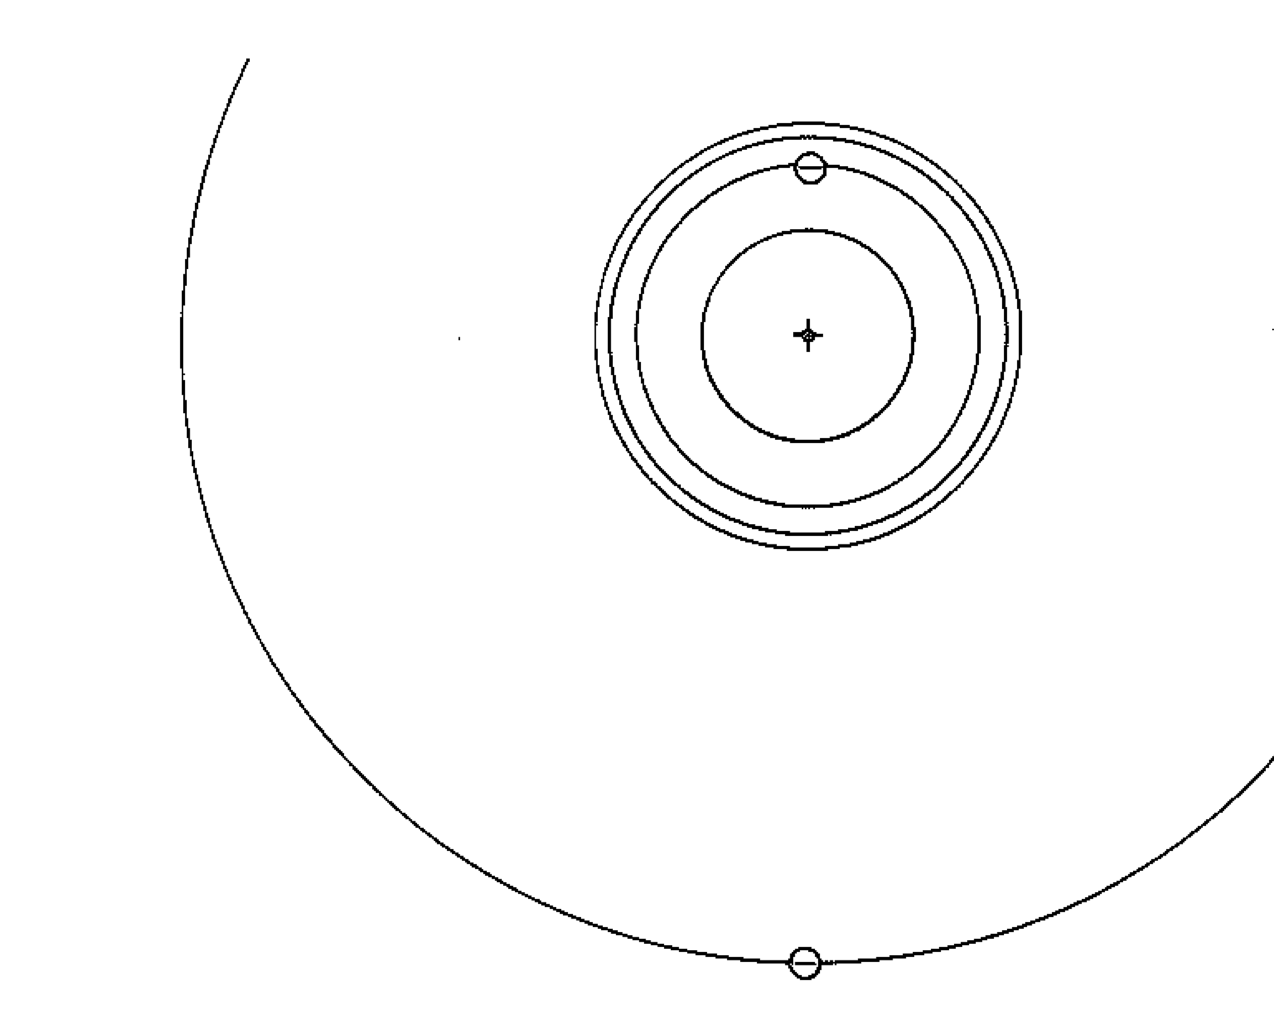
\includegraphics[width=\linewidth]{figs/classicalbohr.png}
\caption{\label{fig:classical}From \cite{collins1989}, shows a picture of a classical Bohr hydrogen atom with an additional electron bound to form an \h\ ion.}
\end{figure}

It has been rigorously shown that \h\ has no bound excited states, i.e., the only bound state is the ground state (\citealt{hill1977}).  As such, \h\ does not have a spectrum as it is normally referred to; there are no electronic transitions between bound states that absorb and emit photons of specific wavelengths.  Its main contribution to the opacity of the solar atmosphere is through continuum absorption of photons with energy greater than the binding energy of its least bound electron.  

The effect of screening due to free electrons on the binding energy of the \h\ ion has been looked at.  The partially ionized nature of the solar atmosphere makes this a relevant study.  \cite{phelpsbajaj1983} use a variational approach to show that the effect screening due to free electrons has on the binding energy of the \h\ ion is within a factor of 2 (as they quantify it) of the effect of screening on the binding energy of a single-electron H atom, despite the electron of the neutral H being $\sim 18$ times more bound than the least bound electron of \h.  To be specific, \cite{phelpsbajaj1983} 
%define a screening parameter $\delta$, where
%\beq
%\delta^2 = \sum_i \frac{4\pi n e^2}{k_B T}\left[ \frac{F_{-1/2}(\nu_i)}{F_{1/2}(\nu_i)}
%\eeq
assume a Dingle-Mansfield screening, which modifies equation~\ref{eq:H} to
\beq
H = \frac{p_1^2 + p_2^2}{2m_e} - \frac{1}{4\pi\epsilon_0}\frac{e^2}{r_1}e^{-\delta r_1} -  \frac{1}{4\pi\epsilon_0}\frac{e^2}{r_2}e^{-\delta r_2} + \\
 \frac{1}{4\pi\epsilon_0}\frac{e^2}{r_{12}} e^{-\delta r_{12}}
\eeq
where $\delta$ is a screening parameter defined in the text.  For my
purpose of comparison the exact definition of the screening parameter
is not necessary to include.  Their results are shown in
figure~\ref{fig:screening}.  They calculate that for  \h\ the binding energy goes to zero for $a_0 \delta = 0.87$  (where $a_0$ is the Bohr radius) while it is shown elsewhere that for H binding energy goes to zero for $a_0 \delta = 1.2$ (\citealt{rogersetal1970}).  The two values of $a_0 \delta$ are not very different which, as mentioned previous, seems surprising due to the factor $~18$ discrepancy between the binding energies of H and \h.  \cite{phelpsbajaj1983} attribute this to the assumption that the interactions between the proton and the electrons and the interaction between the electrons themselves are modified in the presence of free electrons and so the ground state energy is itself modified as a function of $\delta$; so the binding energy is modified both by the presence of free electrons and by the change in the ground state energy in the presence of free electrons.  The interplay of these two effects is what allows a perhaps intially surprisingly large value of $a_0 \delta$ for the binding energy to go to zero in \h.
\begin{figure}
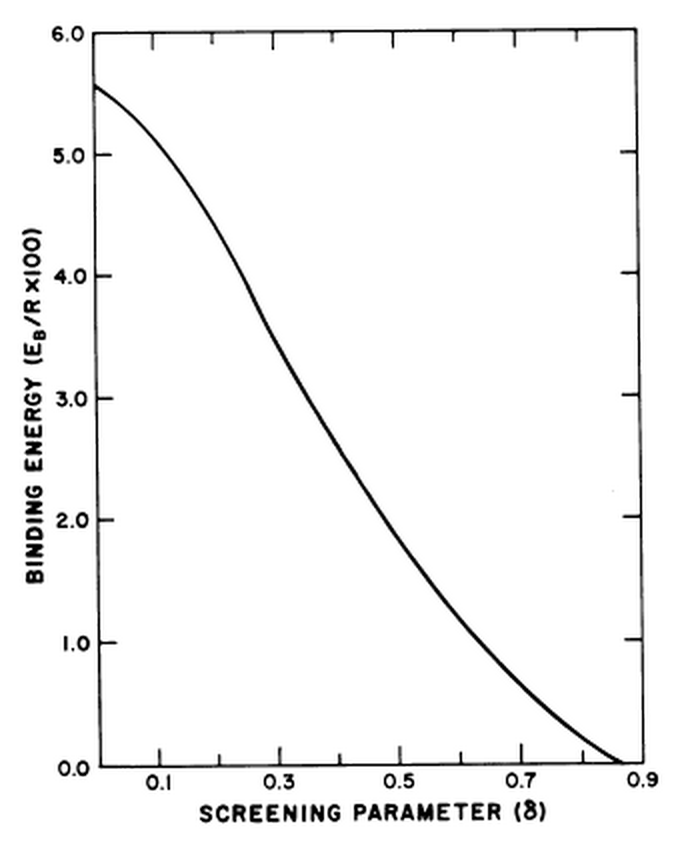
\includegraphics[width=76mm]{figs/screeningparameter.png}%normal width
                                %is 80mm
\caption{\label{fig:screening}Binding energy of the least bound
electron in the \h\ ion as a function of screening parameter
$\delta$.  Binding energy is given in units of the Rydberg energy and
multiplied by 100 (\citealt{phelpsbajaj1983}).}
\end{figure}
